% !TeX program = pdflatex
\documentclass[12pt,a4paper]{article}

% =====================================
%        USTAWIENIA I PAKIETY
% =====================================
\usepackage[utf8]{inputenc}
\usepackage[T1]{fontenc}
\usepackage[polish]{babel}
\usepackage{graphicx}
\usepackage{amsmath, amssymb}
\usepackage{float}
\usepackage{geometry}
\usepackage{booktabs}
\usepackage{caption}
\usepackage{subcaption}
\usepackage{pgfplots}
\usepackage{hyperref}
\geometry{margin=2.5cm}
\setlength{\parindent}{1.2cm}
\setlength{\parskip}{0.5em}
\linespread{1.2}

\pgfplotsset{compat=1.18}

% =====================================
%          DOKUMENT
% =====================================
\begin{document}
	
	% =====================================
	%          STRONA TYTUŁOWA
	% =====================================
	\begin{titlepage}
		\centering
		\large
		\textbf{POLITECHNIKA GDAŃSKA}\\
		Wydział Elektoniki, Telekomunikacji i Informatyki\\[1cm]
		
		\Huge \textbf{Sprawozdanie z ćwiczeń laboratoryjnych}\\[0.3cm]
		\Large z przedmiotu: \textit{Sterownaie Analogowe}\\[1cm]
		
		\begin{tabular}{|p{6cm}|p{8cm}|}
			\hline
			\textbf{Numer ćwiczenia:} & 1 \\
			\hline
			\textbf{Tytuł ćwiczenia:} & Identyfikacja obiektów dynamicznych \\
			\hline
			\textbf{Imię i nazwisko:} & 
			\begin{tabular}[t]{@{}l@{}}
				Mateusz Kuczerowski\\
				Kewin Kisiel\\
			\end{tabular} \\
			\hline
			\textbf{Data pomiarów:} & 9.10.2025 \\
			\hline
			\textbf{Data oddania:} & [dd.mm.rrrr] \\
			\hline
			\textbf{Ocena:} & \\
			\hline
		\end{tabular}\\[1cm]
		
		\vfill
		\textbf{Prowadzący:} dr inż. Piotr Fiertek\\[0.2cm]
		\textbf{Grupa laboratoryjna:} 1A\\[1cm]
		
		\vfill
		Gdańsk, \today
	\end{titlepage}
	
	% =====================================
	%          CEL ĆWICZENIA
	% =====================================
	\section{Cel ćwiczenia}
		Celem ćwiczenia jest ilustracja częstotliwościowych i czasowych metod identyfikacji obiektów
		dynamicznych. 
	
	% =====================================
	%          OPIS POMIARÓW
	% =====================================
	
	\section{Opis wykonywanych czynności}
	W trakcie labolatorium najpierw dokonaliśmy pomiaru odpowiedzi skokowej danego 
	układu następnie doknoaliśmy zmierzenia amplitudy sygnału wyjściowego oraz przesunięcia fazowego między sygnałem wejściowym a wyjściowym dla kilki wybranych częstotliwości.
	
	% =====================================
	%         UKŁADY POMIAROWE
	% =====================================
	
	\section{Układy pomiarowe}
	
 	\quad Zdjęcie pomiarów przeprowadzonych w trakcie labolatorium.
	
	\subsection{Układ inercyjny pierwszego rzędu}
		Transmitancja operatorowa:
		\begin{equation}
			G(s) = \frac{k_p}{1 + sT_p}
		\end{equation}
	
	\noindent Odpowiedź układu na skok jednostkowy:
		\begin{equation}
			h(t) = k_p(1-e^{\frac{-t}{T_p}})\mathbf{1}(t)
		\end{equation}
		
	\noindent	poniżej przedstawiona jest odpowiedź skokowa układu:
		\begin{figure}[H]
			\centering
			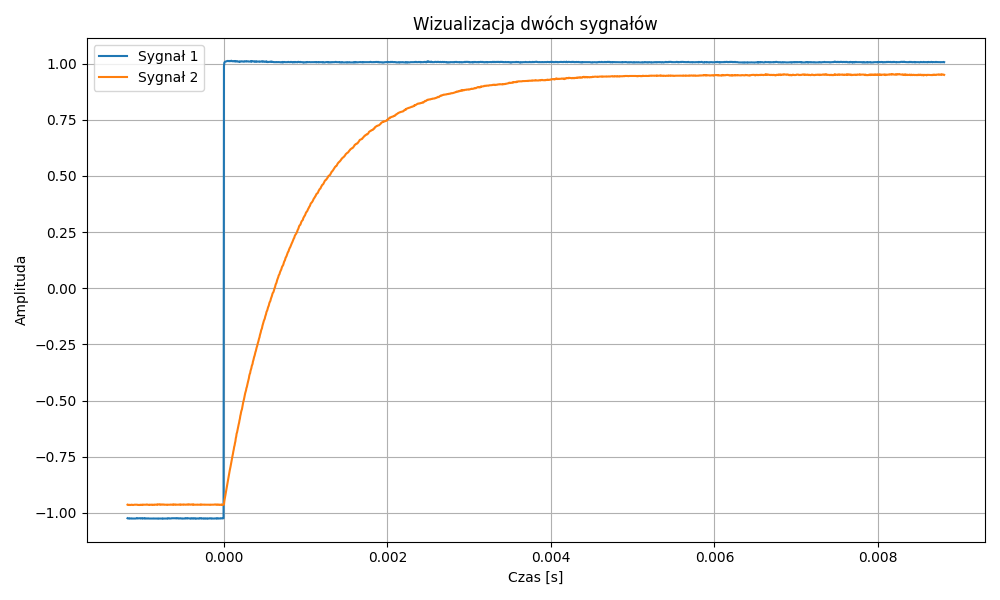
\includegraphics[width=1\textwidth]{zdjecia/Figure_1.png}
			\caption{Odpowiedź układu na skok jednostkowy.}
			\label{fig:odp_na_skok_uk1rz}
		\end{figure}
		
	\subsection{Układ inercyjny pierwszego rzędu z opóźnieniem transportowym}	
	
	\subsection{Układ całkujący}
	
	\subsection{Układ drugiego rzędu}
	
	\subsection{Układ nieminiamlnofazowy}
	
	\begin{equation}
		G(s) = \frac{test}{1 + test}
	\end{equation}
	
	% =====================================
	%          PODSUMOWANIE
	% =====================================
	\section{Podsumowanie}
	Ćwiczenie pozwoliło zapoznać się z analizą odpowiedzi skokowej i porównaniem modelu teoretycznego z rzeczywistym układem.
	
	% =====================================
	%          BIBLIOGRAFIA
	% =====================================
	\begin{thebibliography}{9}
		\bibitem{skrypt} Skrypt do ćwiczeń laboratoryjnych z [nazwa przedmiotu], Politechnika [nazwa], 2025.
		\bibitem{ogata} Ogata K., \textit{Modern Control Engineering}, Prentice Hall.
	\end{thebibliography}
	
\end{document}
